% !TeX root = main.tex

\newcommand{\trait}[1]{
\vspace{.2cm} #1 \line(1,0){30}

	\begin{tabular}{p{0em}p{0em}p{0em}p{0em}p{0em}p{0em}p{0em}p{0em}p{0em}}

		\ding{108} & \ding{109} & \ding{109} & \ding{109} & \ding{109} & \ding{109} & \ding{109} & \ding{109} & \ding{109}  \\
		\ding{111} & \ding{111} & \ding{111} & \ding{111} & \ding{111} & \ding{111} & \ding{111} & \ding{111} & \ding{111}  \\
	\end{tabular}

}

		\newcommand{\shortline}{\line(1,0){22}}	
		\newcommand{\weeline}{\line(1,0){30} \hspace{.6cm}}
		\newcommand{\vlongline}{\line(1,0){100}\hspace{0.8cm}}
		\newcommand{\writeline}{\line(1,0){59}}
\newcommand{\fiveboxes}{\ding{111}\ding{111}\ding{111}\ding{111}\ding{111}}
\newcommand{\threeboxes}{\ding{111}\ding{111}\ding{111}}
\newcommand{\threecircles}{\ding{109}\ding{109}\ding{109}}
\newcommand{\tenboxes}{	\ding{111} & \ding{111} & \ding{111} & \ding{111} & \ding{111} & \ding{111} & \ding{111} & \ding{111} & \ding{111} & \ding{111}  \\}
\newcommand{\tencircles}{\ding{109} & \ding{109} & \ding{109} & \ding{109} & \ding{109} & \ding{109} & \ding{109} & \ding{109} & \ding{109} & \ding{109}  \\}
\newcommand{\attributecircles}{\ding{175}\ding{174}\ding{173}\ding{172}{\Large\ding{109}}\ding{172}\ding{173}\ding{174}\ding{175}}
\newcommand{\Split}{
	\line(1,0){120}

	}
\newcommand{\skill}[1]{#1 & \ding{109} & \ding{109} & \ding{109} \\
}
\newcommand{\sskill}[1]{#1 & \ding{109} & \ding{109} & \ding{109}\\
& \ding{111} & \ding{111} & \ding{111} \\
}

\pagestyle{empty}

\begin{tcbposter}[
  coverage = {
      spread,
      %interior style={bottom color=white},
      watermark text={BIND},
      watermark color=black!25!white,
      watermark opacity=0.4
  },
  poster   = {showframe=false,columns=11,rows=12},
  boxes    = {
      enhanced standard jigsaw,sharp corners=downhill,arc=7mm,boxrule=.6mm,
      colback=white,opacityback=0.7,colframe=black,
      title style={left color=black,right color=white},
      fonttitle=\bfseries
   }
]

%----
% try removing 'interior engine'
\posterbox[blankest,interior engine=path, halign=center,valign=center,colupper=white!25!black,
	]{name=title,column=1,span=11,below=top}{
		\vspace{.3cm}
		\begin{tabular}{llllll}
			Name: & \vlongline & Player: & \vlongline & Code: & \vlongline \\
			\\
			Concept: & \vlongline & Race: & \vlongline & Culture: & \vlongline \\
		\end{tabular}
		\vspace{0.3cm}
}


%----
	\posterbox[adjusted title=Attributes]{name=attributes,column=1,row=2,span=4,rowspan=2}{\vspace{-.3cm}\begin{tabular}{ll}
		& {\tiny Penalties \hspace{1cm} Bonuses} \\
		Strength & \attributecircles \\
		Dexterity & \attributecircles \\
		Speed & \attributecircles \\
		Intelligence & \attributecircles \\
		Wits & \attributecircles \\
		Charisma & \attributecircles \\
	\end{tabular}}
%----

	\posterbox{name=gumption,column=5,row=2,span=3,rowspan=2}{

	\vspace{.2cm} {\small HP}

	\begin{tabular}{p{0em}p{0em}p{0em}p{0em}p{0em}p{0em}p{0em}p{0em}p{0em}p{0em}}

		\ding{108} & \ding{109} & \ding{109} & \ding{109} & \ding{109} & \ding{109} & \ding{109} & \ding{109} & \ding{109} & \ding{109}  \\
		\tenboxes
	\end{tabular}

	\vspace{.6cm} {\tiny Fatigue}

	\begin{tabular}{p{0em}p{0em}p{0em}p{0em}p{0em}p{0em}p{0em}p{0em}p{0em}p{0em}}

	\tenboxes
		\ding{111} & \ding{111} & \ding{111} & \ding{111} & \ding{111} \\
		\ding{182} & \ding{183} & \ding{184} & \ding{185} & \ding{186} & \\
	\end{tabular}

	}
%----
	\posterbox{name=mp,column=8,row=2,span=3,rowspan=2}{

		\vspace{.2cm} {\small FP} \shortline {\tiny $+ Cha$}

	\begin{tabular}{p{0em}p{0em}p{0em}p{0em}p{0em}p{0em}p{0em}p{0em}p{0em}p{0em}}

		\tencircles
		\tenboxes
		\tencircles
		\tenboxes
	\end{tabular}

		\vspace{.2cm} {\small MP} \line(1,0){30} {\tiny $+Int$}

	\begin{tabular}{p{0em}p{0em}p{0em}p{0em}p{0em}p{0em}p{0em}p{0em}p{0em}}

	\ding{109} & \ding{109} & \ding{109} & \ding{109} & \ding{109} & \ding{109} & \ding{109} & \ding{109} & \ding{109}  \\
		\ding{111} & \ding{111} & \ding{111} & \ding{111} & \ding{111} & \ding{111} & \ding{111} & \ding{111} & \ding{111}  \\
	\end{tabular}



		}

%----
		\posterbox{name=track,column=11,row=1,span=1,rowspan=12}{ 
			{\large

			\tracker
			\tracker
			\tracker
			\tracker
			\tracker
			\tracker
			\tracker
			\tracker
			\tracker
			\tracker
			\tracker
			\tracker
			\tracker
			\tracker
			\tracker
			\tracker
			\tracker
			\tracker


			}

			}

%----

		\posterbox[adjusted title=Damage]{name=track,column=1,row=4,span=2,rowspan=1}{ 

}

%----

	\posterbox[blankest]{name=factors,column=1,row=4,span=0,rowspan=0}{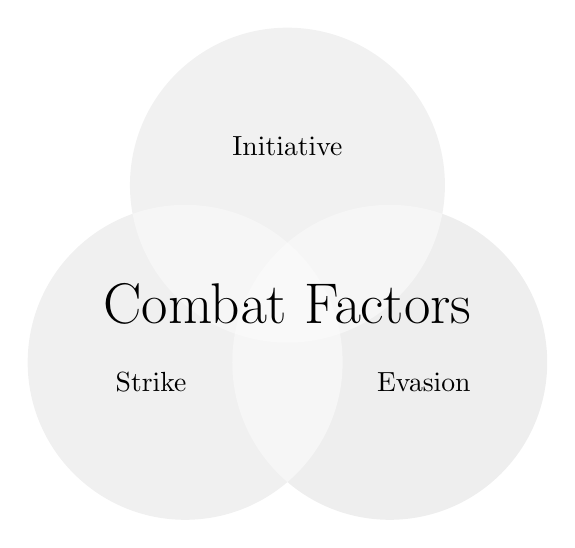
\begin{tikzpicture}
  \begin{scope}[blend group = soft light]
    \fill[gray!11!white]   ( 90:1.5) circle (2);
    \fill[gray!12!white] (210:1.5) circle (2);
    \fill[gray!13!white]  (330:1.5) circle (2);
  \end{scope}
  \node at ( 90:2)    {Initiative};
  \node at ( 210:2)   {Strike};
  \node at ( 330:2)   {Evasion};
  \node [font=\huge] {Combat Factors};
\end{tikzpicture}}

%----

	\posterbox{name=initbox,column=1,row=7,span=3.7,rowspan=1.1}{\begin{multicols}{2}{\tiny \begin{tabular}{lc}
		{\bf Action} & {\bf Cost} \\\hline
		Med. Weapon & 6 \\
		Light Weapon & 4 \\
		Draw Weapon & 2 \\
		Projectile & 4 \\
		Use Item & 8 \\
		Spell & 3+lv. \\
		
	\end{tabular}}
		{\tiny \begin{tabular}{lc}
		{\textbf Quick Actions} & \\\hline
		Defence & 2 \\
		Guard & 2 \\
		Keep Edgy & 2 \\
		Move & 2 \\
		Speak & 2 \\
		\end{tabular}}

	\end{multicols}
}
%----

	\posterbox[adjusted title=Abilities \& Specializations]{name=racial_abilities,column=5,row=7,rowspan=1,span=6}{}

%----
	\posterbox[adjusted title=Armoury]{name=armoury,column=5,row=4,span=6,rowspan=3}{
		\begin{tabular}{p{.2\textwidth}lllll}
			Weapon & Dam. & Init. & Ev. & Wt. & Knack \\
			\\
			
			\writeline & \shortline & \shortline & \shortline &\shortline &  \writeline \\
			\writeline & \shortline & \shortline & \shortline &\shortline &  \writeline \\
			\writeline & \shortline & \shortline & \shortline &\shortline &  \writeline \\
			\writeline & \shortline & \shortline & \shortline &\shortline &  \writeline \\
			\writeline & \shortline & \shortline & \shortline &\shortline &  \writeline \\
			\writeline & \shortline & \shortline & \shortline &\shortline &  \writeline \\
		\end{tabular}	
		\vspace{.3cm}

		\begin{tabular}{lcccc}
			Armour & DR & Weight & Type & Encumbrance \\
			\\
			\writeline & \shortline & \shortline & \shortline & \shortline \\
		\end{tabular}

	}
%----
	\posterbox[adjusted title=Skills]{name=skills,column=8,row=8,span=3.1,rowspan=4.8}{
		\begin{tabular}{lp{0em}p{0em}p{0em}}
			\sskill{Combat*}
			\sskill{Projectiles*}
			& \\
			\skill{Academics*}
			\sskill{Athletics}
			\skill{Beast Ken*}
			\sskill{Crafts*}
			\skill{Deceit}
			\skill{Empathy}
			\skill{Medicine*}
			\skill{Performance*}
			\skill{Larceny}
			\skill{Stealth}
			\sskill{Survival*}
			\skill{Tactics*}
			\skill{Vigilance}
			\skill{\line(1,0){70}}
			\sskill{\line(1,0){70}}



		\end{tabular}
	}

	\posterbox[adjusted title=Spheres]{name=spheres,column=1,row=8,span=3.8,rowspan=2}
	{\vspace{.2cm} \line(1,0){110} \fiveboxes

\vspace{.2cm} \line(1,0){110} \fiveboxes

\vspace{.2cm} \line(1,0){110} \fiveboxes

\vspace{.2cm} \line(1,0){110} \fiveboxes

	}

%----

	\posterbox[adjusted title=Equipment]{name=equipment,column=1,row=10,span=7,rowspan=2.8}{

		\newcommand{\longline}{\line(1,0){340}\par\vspace{.2cm}}
		\vspace{.4cm}

	\longline	

	\longline	

	\longline	

	\longline	

	\longline	

	\longline	

	\longline	

	CP \weeline SP\weeline GP\weeline}

	\posterbox[adjusted title=Knacks]{name=knacks,column=5,row=8,span=3,rowspan=2}{
		\vspace{.3cm}

		\Split
		\Split
		\Split
		\Split
		\Split
		\Split

	}
\end{tcbposter}

\pagebreak

\begin{tcbposter}[
  coverage = {
      spread,
      %interior style={bottom color=white},
      watermark text={stories \\ companions \\ notes},
      watermark color=black!25!white,
      watermark opacity=0.4
  },
  poster   = {showframe=false,columns=11,rows=12},
  boxes    = {
      enhanced standard jigsaw,sharp corners=downhill,arc=7mm,boxrule=.6mm,
      colback=white,opacityback=0.7,colframe=black,
      title style={left color=black,right color=white},
      fonttitle=\bfseries
   }
]

	\posterbox[adjusted title=Stories]{name=stories,column=1,row=1,rowspan=11,span=11}{

		{\Huge Story Points}

		\vspace{0.5cm}

	\begin{tabular}{p{1em}p{1em}p{1em}p{1em}p{1em}p{1em}p{1em}}

		\Huge\ding{111} & \Huge\ding{111} & \Huge\ding{111} & \Huge\ding{111} & \Huge\ding{111} & \huge\ding{111} & \Large\ding{111} \\

	\end{tabular}

		}
\end{tcbposter}

